\subsection{Register Directory}
\begin{figure}[H]
	\centering
	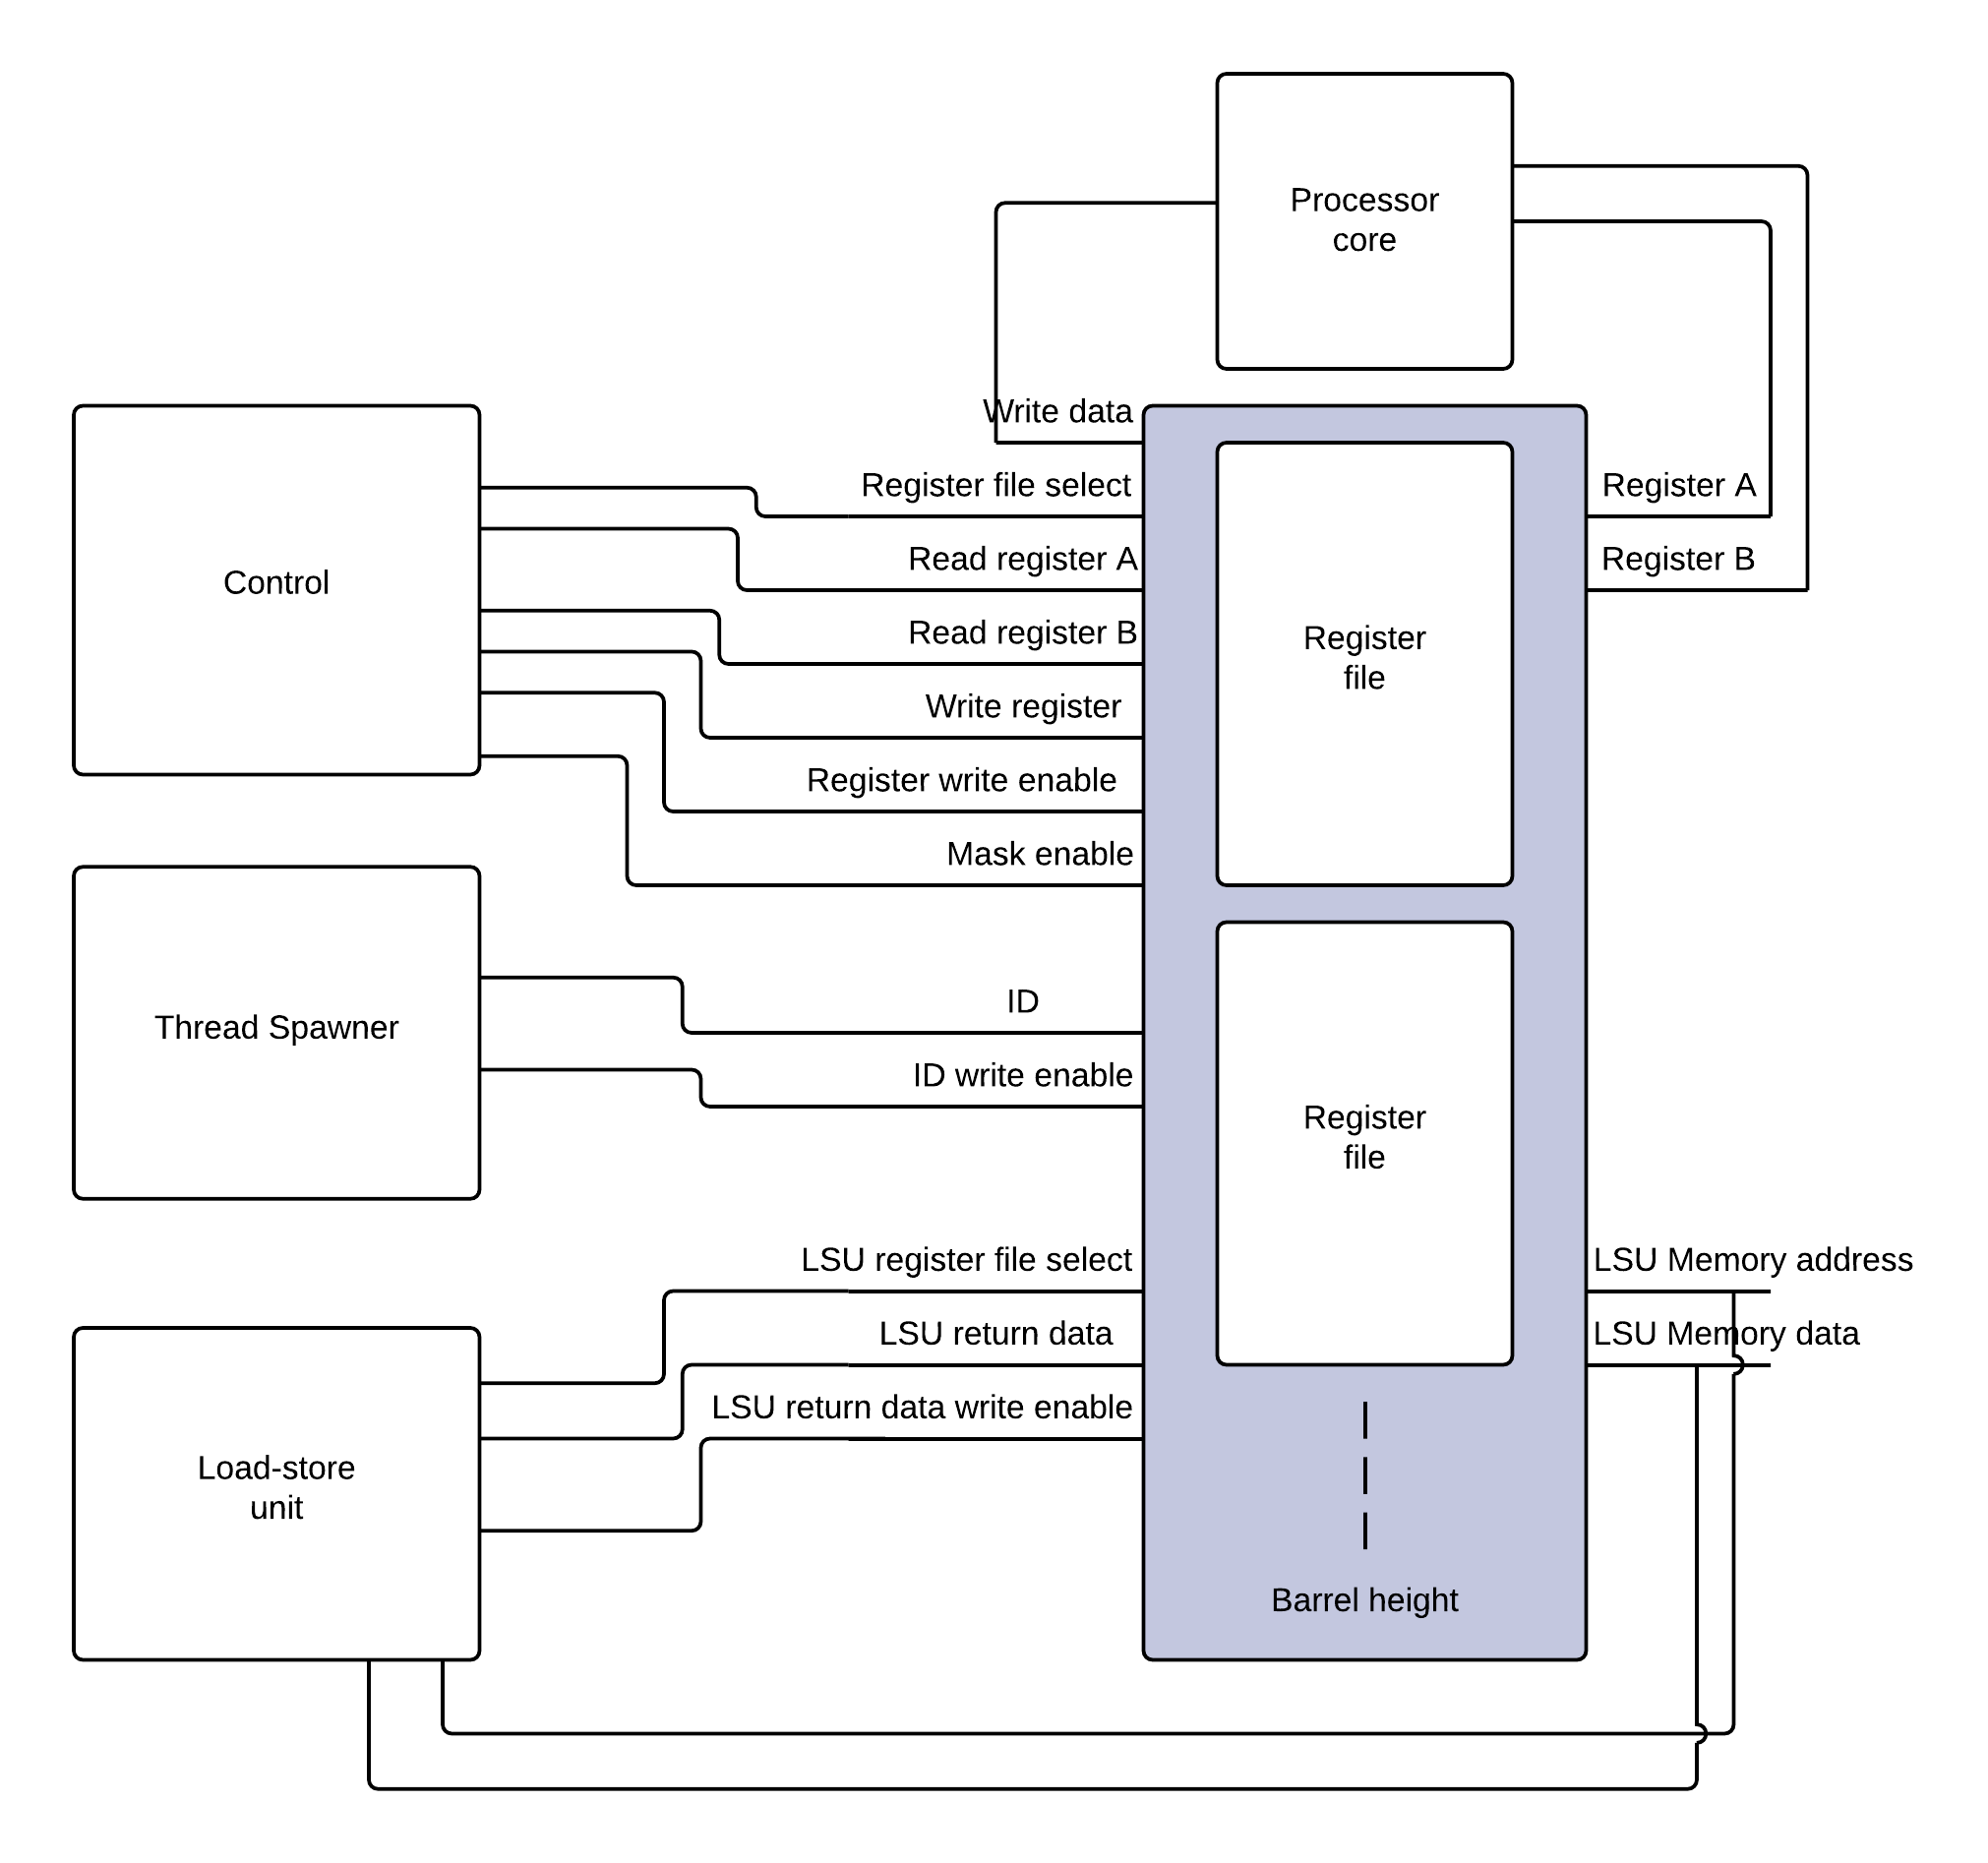
\includegraphics[width=\textwidth]{../gpu/diagrams/register_directory.png}
	\caption{The register directory, and its neighboring components.}
	\label{fig:register_directory}
\end{figure}

There is one register directory per processor core.
Each register directory contains one register file per barrel row.
The register files include seven dedicated registers, and nine general purpose registers (Table \ref{tab:registers_overview}).

\begin{table}[H]
	\centering
	\begin{tabular}{|c|c|c|}
		\hline Register number & Description & RW \\ 
		\hline \$0 & Zero register & Read-only \\ 
		\hline \$1 & ID High & Read/Write \\ 
		\hline \$2 & ID Low & Read/Write \\ 
		\hline \$3 & Address High & Read/Write \\ 
		\hline \$4 & Address Low & Read/Write \\ 
		\hline \$5 & LSU data & Read/Write \\ 
		\hline \$6 & Masking register & Read/Write \\ 
		\hline \$7 - \$15 & General purpose registers & Read/Write \\ 
		\hline 
	\end{tabular} 
	\caption{The registers contained within the register files.}
	\label{tab:registers_overview}
\end{table}

Individual register files are selected by using the \emph{register file select} signal.
The register file select signal is set by the barrel select component.
Within the register directory, the other input signals are routed to the selected register file using the select signal.
Consequently, from the processor core's point of view, there's just one register file.

The dedicated registers serve special purposes in the architecture.
Often, the processor core will be accessing a register file and at the same time, other components may also need access the same, or a different, register file.
To solve this, the special registers are given dedicated signals that the other components use for reading/writing to the register file.
Ignoring registers \$0 and \$6, the rest of the dedicated registers may be used as general purpose registers.
Using them at the same time as other components are accessing them will result in undefined behavior, and is left as the programmer's responsibility.

The masking register is used to enable conditional execution.
If masking is enabled the first bit of masking register is used to disable writes to the register file, making the instruction have no effect (Figure \ref{fig:masking}).
\begin{figure}[H]
	\centering
	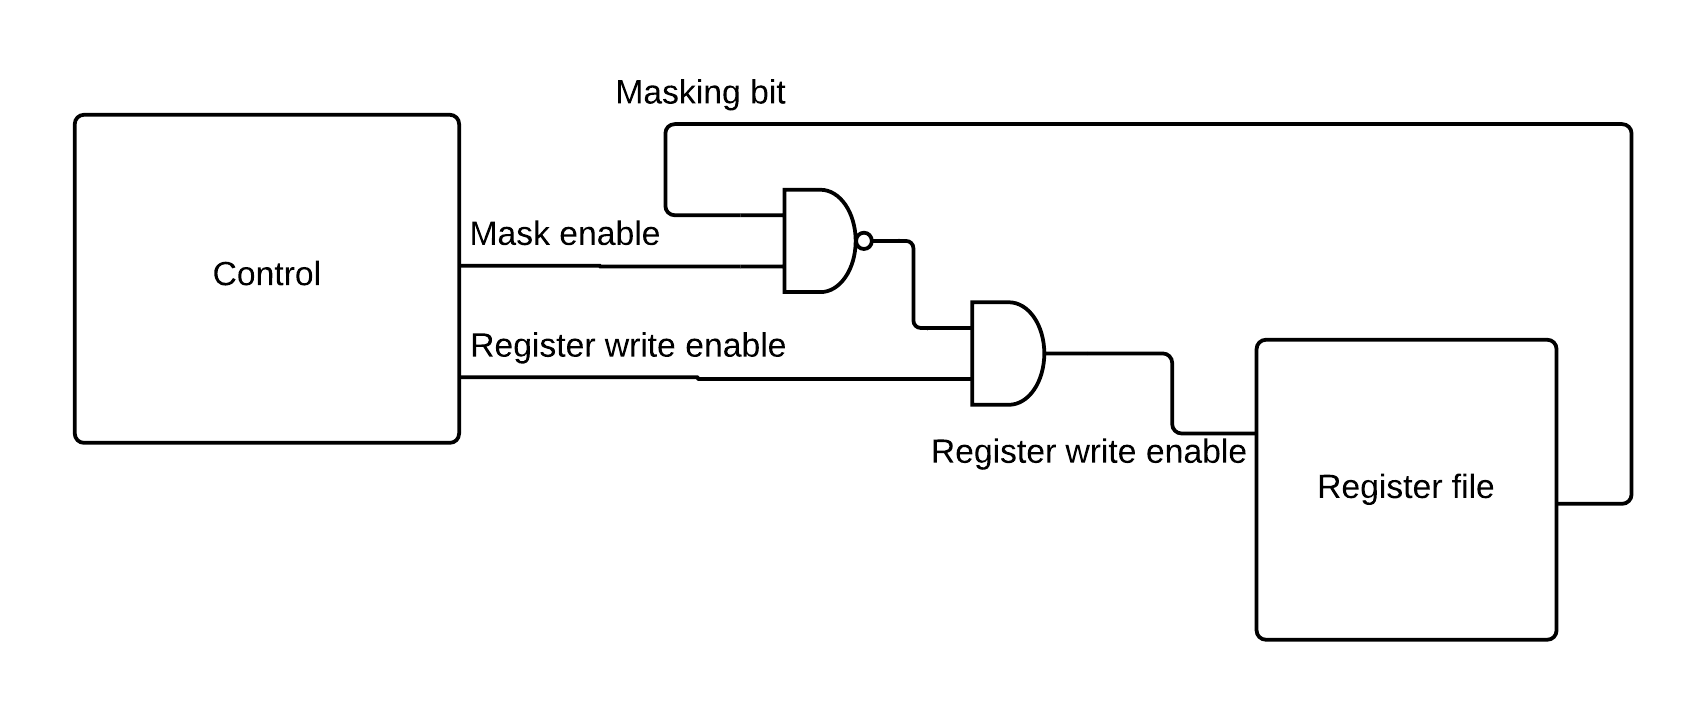
\includegraphics[width=0.8\textwidth]{../gpu/diagrams/masking.png}
	\caption{Using the mask bit to disable register writes.}
	\label{fig:masking}
\end{figure}

Data memory addresses are 20 bit wide, and thread IDs are 19 bit wide.
Registers can only store 16 bit values.	
To represent these values they are split into registers which contain the higher and lower bits.

The load store unit (LSU) has a separate signal for selecting register files.
Using the signal, the LSU can write data loaded from memory into the register files on its own.
